\documentclass[10pt,landscape]{article}
\usepackage{multicol}
\usepackage{calc}
\usepackage{ifthen}
\usepackage[landscape]{geometry}
\usepackage{amsmath,amsthm,amsfonts,amssymb}
\usepackage{color,graphicx,overpic}
\usepackage{hyperref}


\pdfinfo{
  /Title (example.pdf)
  /Creator (TeX)
  /Producer (pdfTeX 1.40.0)
  /Author (Seamus)
  /Subject (Example)
  /Keywords (pdflatex, latex,pdftex,tex)}

% This sets page margins to .5 inch if using letter paper, and to 1cm
% if using A4 paper. (This probably isn't strictly necessary.)
% If using another size paper, use default 1cm margins.
\ifthenelse{\lengthtest { \paperwidth = 11in}}
    { \geometry{top=.5in,left=.5in,right=.5in,bottom=.5in} }
    {\ifthenelse{ \lengthtest{ \paperwidth = 297mm}}
        {\geometry{top=1cm,left=1cm,right=1cm,bottom=1cm} }
        {\geometry{top=1cm,left=1cm,right=1cm,bottom=1cm} }
    }

% Turn off header and footer
\pagestyle{empty}

% Redefine section commands to use less space
\makeatletter
\renewcommand{\section}{\@startsection{section}{1}{0mm}%
                                {-1ex plus -.5ex minus -.2ex}%
                                {0.5ex plus .2ex}%x
                                {\normalfont\large\bfseries}}
\renewcommand{\subsection}{\@startsection{subsection}{2}{0mm}%
                                {-1explus -.5ex minus -.2ex}%
                                {0.5ex plus .2ex}%
                                {\normalfont\normalsize\bfseries}}
\renewcommand{\subsubsection}{\@startsection{subsubsection}{3}{0mm}%
                                {-1ex plus -.5ex minus -.2ex}%
                                {1ex plus .2ex}%
                                {\normalfont\small\bfseries}}
\makeatother

% Define BibTeX command
\def\BibTeX{{\rm B\kern-.05em{\sc i\kern-.025em b}\kern-.08em
    T\kern-.1667em\lower.7ex\hbox{E}\kern-.125emX}}

% Don't print section numbers
\setcounter{secnumdepth}{0}


\setlength{\parindent}{0pt}
\setlength{\parskip}{0pt plus 0.5ex}

%My Environments
\newtheorem{example}[section]{Example}
% -----------------------------------------------------------------------

\begin{document}
\raggedright
\footnotesize
\begin{multicols}{3}


% multicol parameters
% These lengths are set only within the two main columns
%\setlength{\columnseprule}{0.25pt}
\setlength{\premulticols}{1pt}
\setlength{\postmulticols}{1pt}
\setlength{\multicolsep}{1pt}
\setlength{\columnsep}{2pt}

\begin{center}
     \Large{\underline{Computer Systems {\small Cheat Sheet by David Sha}}} \\
\end{center}

\section{W1: Operating Systems}
\textbf{CPU cycle:} fetch, decode, execute, store.\\
\textbf{Registers:} hold variables and temporary results.\\
\textbf{Special registers:} program counter (PC), stack pointer (SP), program status word (PSW).\\
\textbf{User mode:} restricted access to memory and instructions.\\
\textbf{Kernel mode:} full access to the above.\\
\textbf{Memory stack:}\\
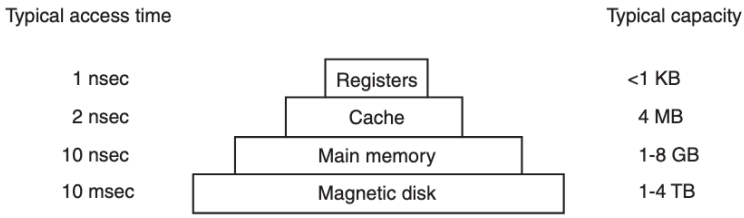
\includegraphics[width=\linewidth]{figs/memory-stack.png}

\subsection{System calls}
\begin{enumerate}
    \item Put system call number in register of OS.
    \item Execute trap instruction (switch to kernel mode).
    \item OS executes system call from fixed address in kernel memory.
    \item The kernel code that starts following the trap instruction is called the \textbf{trap handler}. Trap handler examines the system call number and dispatches the correct system-call handle.
    \item System call handler runs.
    \item Return to user mode.
\end{enumerate}

\section{W2: Processes, Threads}
\textbf{Why processes?} Simultaneous execution of multiple programs on single CPU.\\
\textbf{Why threads?} Simultaneous execution of multiple parts of a program on single CPU. Threads share global variables and heap memory.\\

\subsection{Interprocess communication}
\textit{Process/Thread Synchronization} Race conditions occur when multiple processes/threads access shared data and try to change it at the same time.\\
\textbf{Critical region:} code segment where shared data is accessed.\\
\textbf{Mutual exclusion:} only one process/thread can be in critical region at a time.\\
\begin{enumerate}
    \item No two processes/threads may be simultaneously inside their critical regions.
    \item No assumptions may be made about speeds or the number of CPUs.
    \item No process/thread running outside its critical region may block other processes/threads.
    \item No process/thread should have to wait forever to enter its critical region.
\end{enumerate}

\subsubsection{Possible approaches to mutual exclusion}
\textbf{Busy waiting:} process/thread stays in loop in kernel mode until it can enter critical region. Pros: simple, no context switch. Cons: wastes CPU time, starvation (Priority Inversion Problem).\\
\begin{enumerate}
    \item \textbf{Lock variables:} each process/thread has a lock variable. Process/thread can enter critical region only if its lock variable is 0.\\
    \item \textbf{Strict alternation:} processes/threads take turns entering critical region.\\
    \item \textbf{Peterson's solution:} two processes/threads, two lock variables.\\
    \item \textbf{Test-and-set (TSL):} atomic instruction that sets lock variable to 1 and returns old value.\\
\end{enumerate}

\subsubsection{Deadlocks}
Four conditions for deadlock:
\begin{enumerate}
    \item \textbf{Mutual exclusion:} only one process/thread can use a resource at a time.
    \item \textbf{Hold and wait:} processes/threads hold resources while waiting for others.
    \item \textbf{No preemption:} resources can be released only voluntarily by process/thread holding it.
    \item \textbf{Circular wait:} two or more processes/threads form a circular chain where each process/thread waits for a resource held by next process/thread in chain.
\end{enumerate}
\section{W3: Scheduling, Memory Management}
\textbf{Preemption:} Preemptive scheduling is when the scheduler decides to switch to another process/thread. Clock interrupts used upon a quantum. Non-preemptive scheduling is when the process/thread itself decides to give up the CPU or is blocked.\\
\textbf{Context switch:} Switching from one process/thread to another is expensive.\\

\subsection{Non-preemptive scheduling}
\textbf{First-come, first-served (FCFS):} Simple, but long average waiting time.\\
\textbf{Shortest job first (SJF):} Shortest average waiting time, but long waiting time for long processes/threads. Average turnaround time is minimized.\\

\subsection{Preemptive scheduling}
\textbf{Round-robin (RR):} Each process/thread gets a quantum.\\
\textbf{Shortest remaining time first (SRTF):} Shortest average waiting time, but long waiting time for long processes/threads. Average turnaround time is minimized.\\
\textbf{Priority scheduling:} Each process/thread has a priority. May lead to starvation.\\

\subsection{Memory management}
\textbf{Why Memory Management?} Support multiprogramming. Secure isolation between processes/threads and OS memory. Enables virtual memory which allows processes/threads to use more memory than is physically available.\\
\textbf{No memory abstraction:} Use swap space on disk. Multiplex physical memory.\\

\subsubsection{Memory abstraction}
\textbf{Logical address space:} set of addresses that a process/thread can use which are mapped to physical addresses.\\
\textbf{Base and limit registers:} base register holds start address of process/thread, limit register holds size of process/thread.\\
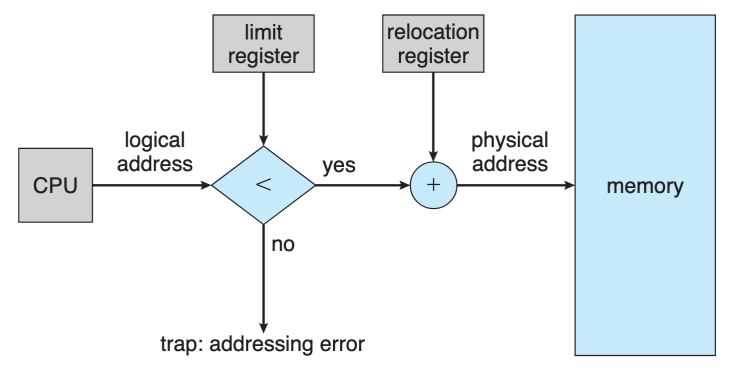
\includegraphics[width=\linewidth]{figs/base-and-limit-registers.png}
\textbf{Memory management unit (MMU):} hardware device that maps logical addresses to physical addresses.\\
\textbf{Manage free memory:} using bitmap or linked list.\\
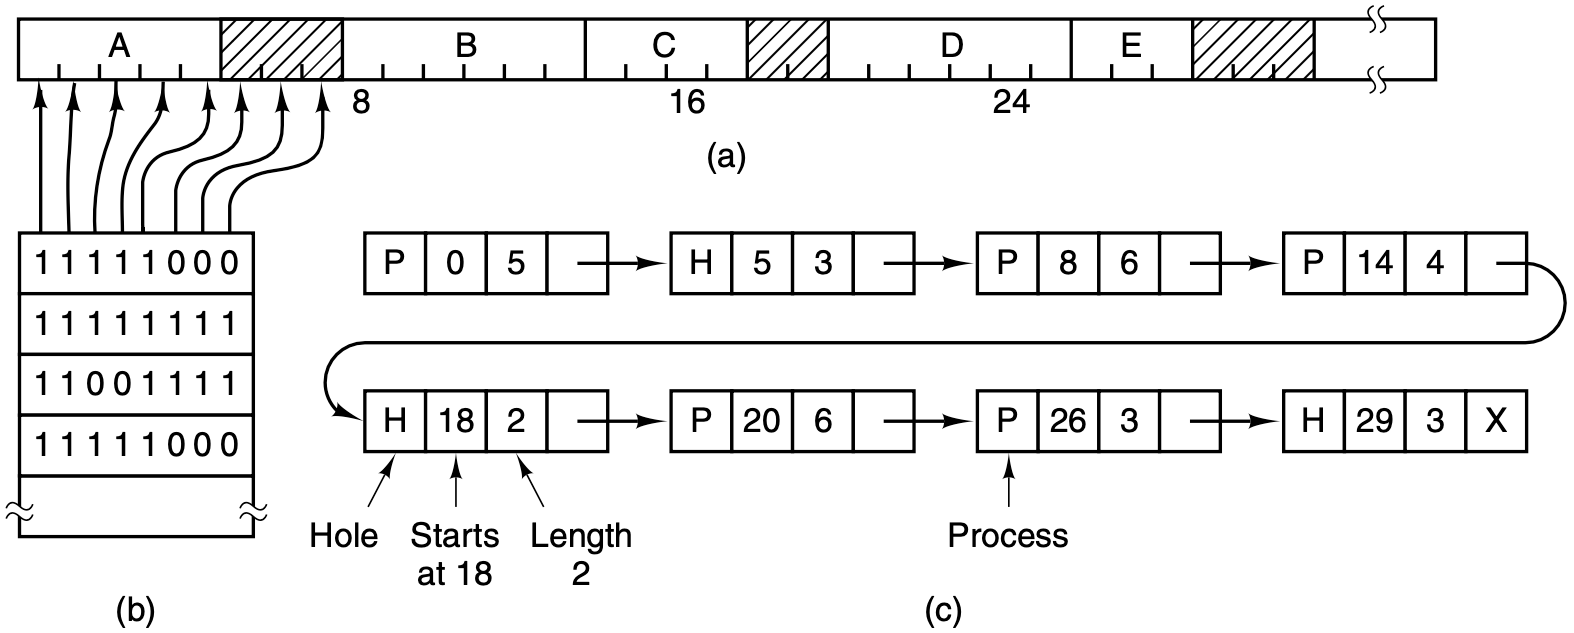
\includegraphics[width=\linewidth]{figs/memory-management.png}

\subsubsection{Virtual memory}
\textbf{Why virtual memory?} Processes/threads can use more memory than is physically available.\\
\textbf{Page table:} maps virtual pages to physical pages.\\
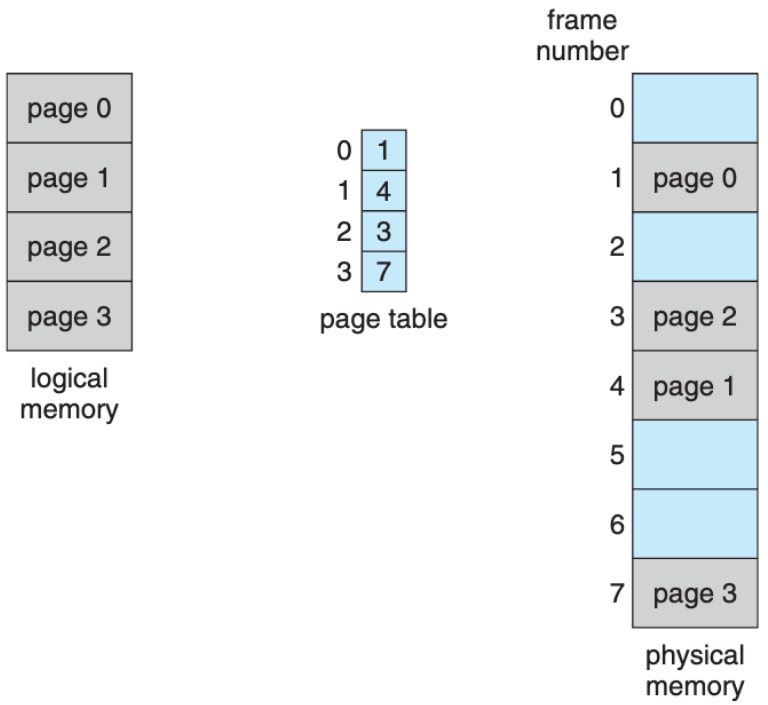
\includegraphics[width=0.4\linewidth]{figs/paging-model.png}
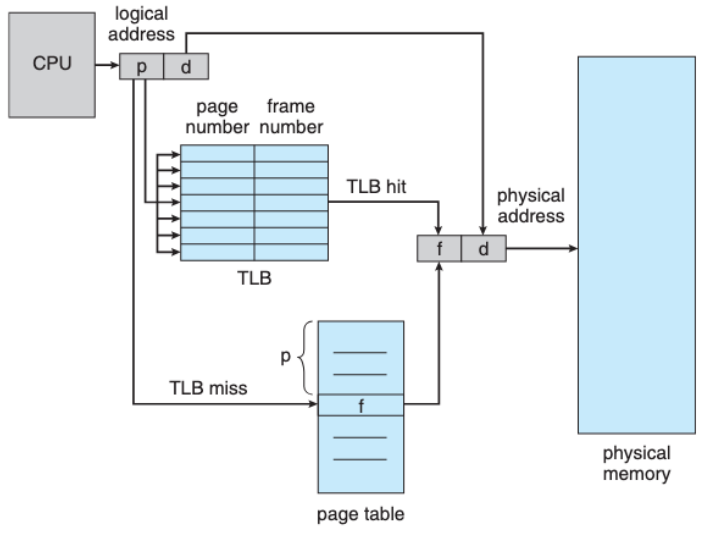
\includegraphics[width=0.45\linewidth]{figs/mmu-with-tlb.png}\\
\textbf{Translation Lookaside Buffer (TLB):} cache for page table, faster than main memory, speeds up address translation.\\
\textbf{Page replacement algorithms for TLB:} \textit{NRU} (Not Recently Used, R and M bit, 4 classes between referenced and modified).\\

\section{W4: Cryptography}

\section{W5: PKI, Certificates, TLS}

\section{W6: Network Protocols, OSI Layers}
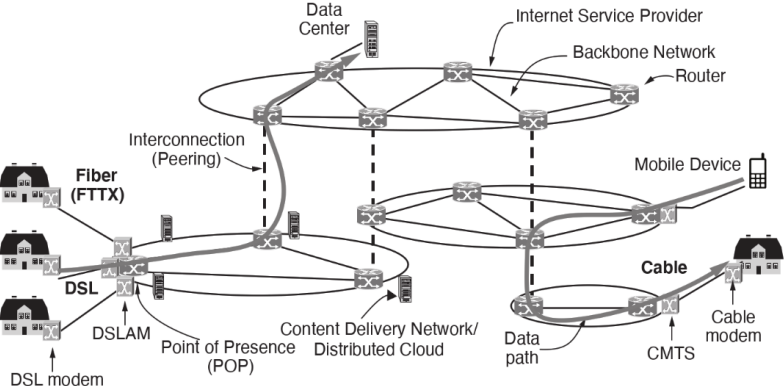
\includegraphics[width=\linewidth]{figs/internet-diagram.png}
\textbf{Two contenders:} TCP/IP and OSI (Open Systems Interconnection). ARPANET used TCP/IP was simpler and won. OSI was too concerned with generality and extensibility.\\
\textbf{OSI model:} is the ideal model that TCP/IP is based on.
\begin{itemize}
    \item A layer should be created where different level of abstraction is needed.
    \item Each layer should perform a well-defined function.
    \item The function of each layer should be chosen with an eye toward defining internationally standardized protocols.
    \item The layer boundaries should be chosen to minimize the information flow across the interfaces.
    \item The number of layers should be large enough that distinct functions need not be thrown together in the same layer out of necessity and small enough that the architecture does not become unwieldy.
\end{itemize}
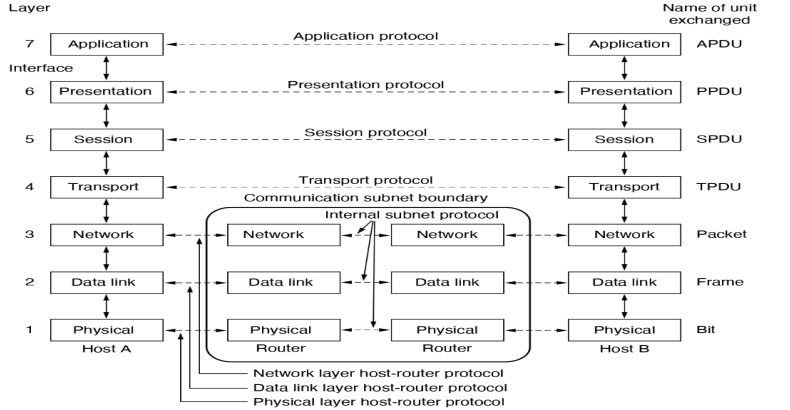
\includegraphics[width=\linewidth]{figs/osi-model.png}

\section{W7: Application Layer}
\textbf{URL/URI:} Uniform Resource Locator/Identifier.\\
{\tiny \verb|scheme:[//[user[:password]@]host[:port]][/path][?query][#fragment]|}\\
\textbf{HTTP:} HyperText Transfer Protocol.\\
\begin{itemize}
    \item \textbf{HTTP/1.0:} one object per TCP connection.
    \item \textbf{HTTP/1.1:} multiple objects per TCP connection/persistent connections.
    \item \textbf{HTTP/2:} multiplexing/asynchronous requests over TCP connection, compression, prioritization.
    \item \textbf{HTTP/3:} QUIC (UDP-based), everything in HTTP/2.
\end{itemize}
\textbf{Domain Name System (DNS):} translates domain names to IP addresses.\\
\begin{itemize}
    \item \textbf{Domain name space:} tree structure, top-level domain (TLD), second-level domain (SLD), subdomain.
    \item \textbf{DNS database:} distributed database storing resource records (RR).
    \item \textbf{Name servers:} each domain has authoritative name server (ANS).
    \item \textbf{Resolvers:} DNS clients that query name servers in response to client requests.
\end{itemize}
\textbf{Mail:} SMTP (Simple Mail Transfer Protocol).\\
\begin{itemize}
    \item \textbf{POP3:} Post Office Protocol v3, download and delete from server.
    \item \textbf{IMAP:} Internet Mail Access Protocol, download without deleting from server. More features than POP3.
    \item \textbf{MIME:} Multipurpose Internet Mail Extensions, allows non-ASCII attachments.
\end{itemize}
\textbf{Remote Procedure Call (RPC):} allows a program to call a procedure on another machine.\\

\section{W8-10: Transport Layer}

\subsection{Transmission Control Protocol (TCP)}
\textbf{Connection-oriented:} three-way handshake.\\
\textbf{Congestion control:} slow start, congestion avoidance, fast retransmit, fast recovery.\\
\textbf{Full duplex:} two-way simultaneous data transfer.\\
\textbf{Sliding window protocol:} sender maintains a window of sent but unacknowledged packets. Reliable data delivery without overloading the receiver.\\
\textbf{TCP headers:} source port, destination port, sequence number (if SYN = 1, initial sequence number. If SYN = 0, sequence number of first data byte in this segment), acknowledgement number (if ACK = 1, next sequence number that the sender of the ACK is expecting), data offset (size of TCP header $20 \text{ bytes} = 5 \times 32 \text{-bits}$ to $60 \text{ bytes} = 15 \times 32 \text{-bits}$), flags (single bit flags), window size (how much data the sender of this segment is willing to receive).\\
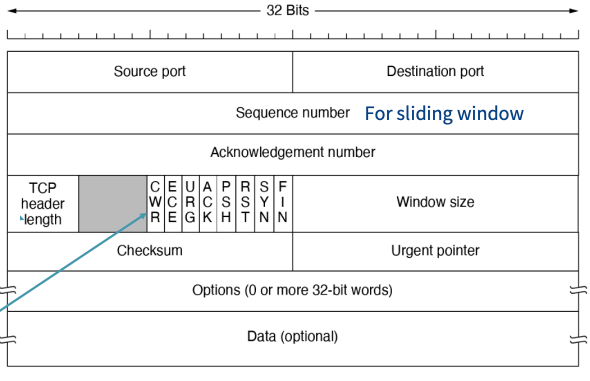
\includegraphics[width=\linewidth]{figs/tcp-header.png}
\textbf{Three-way handshake:} SYN, SYN-ACK, ACK.\\
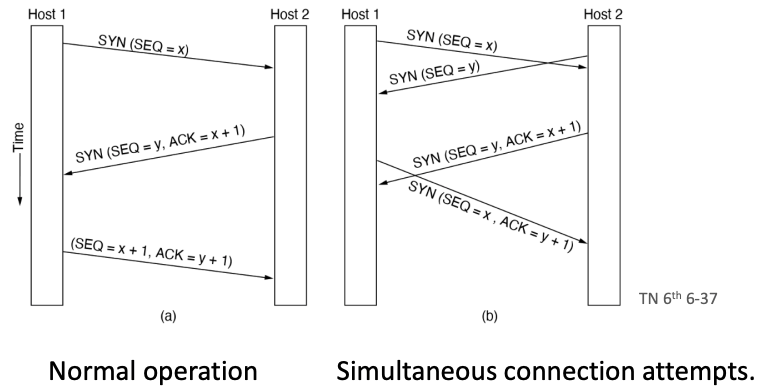
\includegraphics[width=\linewidth]{figs/three-way-handshake.png}

\subsection{TCP flow control}
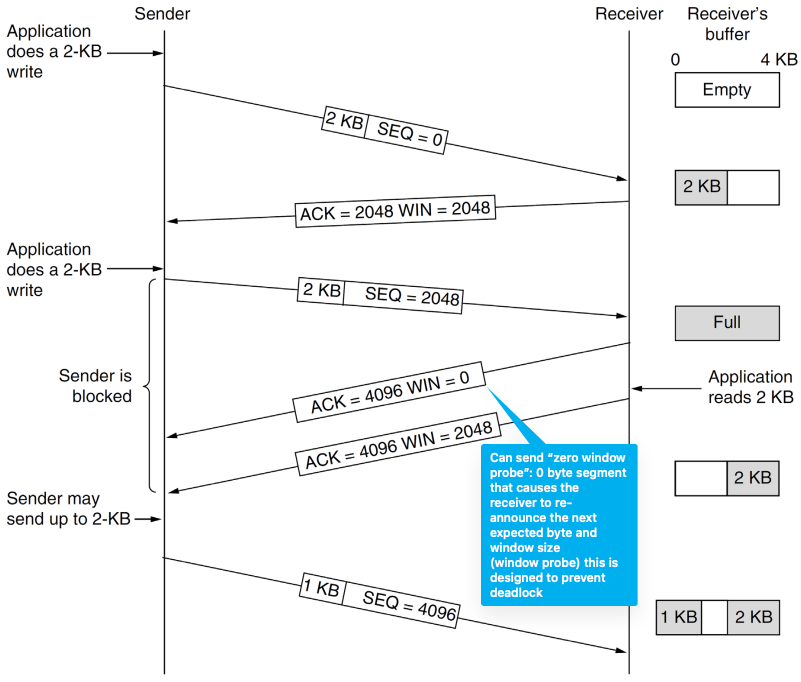
\includegraphics[width=\linewidth]{figs/tcp-sliding-window.png}
\textbf{Go-back-N:} when a packet is lost, retransmit all packets from the lost packet onwards. Receiver does not need to buffer out-of-order packets.\\
\textbf{Selective repeat:} (or fast retransmit) when a packet is lost, retransmit only the lost packet. Receiver needs to buffer out-of-order packets. Only helps if loss is common.\\

\subsection{TCP congestion control}
\textbf{Slow start:} increase congestion window size exponentially until a threshold.\\

\subsubsection{Macroscopic model}
\textbf{Average increase in congestion window size:} $$\frac{(1-p)}{W} - p \frac{W}{2}$$
\textbf{Equilibrium point:} $$\frac{(1-p)}{W} - p \frac{W}{2} = 0 \implies W \approx \sqrt{\frac{2}{p}}$$
\textbf{Rate:} $$\frac{W}{T} \approx \frac{1}{T} \sqrt{\frac{2}{p}} \text{ where } T = \text{round trip time}$$
This means for a given packet loss rate, the rate of increase of congestion window size is inversely proportional to the round trip time.\\

\subsection{Other layers}
\textbf{Presentation layer:} syntax and semantics of information exchanged between hosts.\\
\textbf{Session layer:} synchronization, checkpointing, recovery of data exchange.\\
\textbf{Transport layer:} reliable data transfer, congestion control, flow control.\\
\textbf{Transport layer encapsulation:} abstract representation of messages sent to and from transport entities.\\
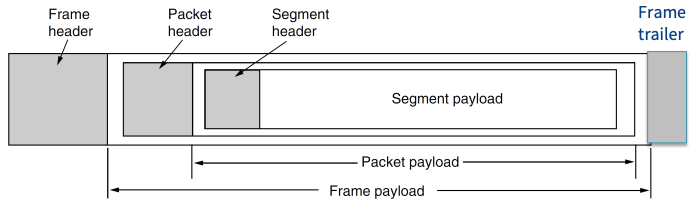
\includegraphics[width=\linewidth]{figs/encapsulation-of-segments.png}\\


\subsection{Packet switching, circuit switching}
\textbf{Packet switching:} a mode of data transmission in which a message is broken into a number of parts which are sent independently, over whatever route is optimum for each packet, and reassembled at the destination. The internet is a packet switched network.\\
\textbf{Packet forwarding (connectionless):} uses packet switching and must have a minimum required service of "send packet". This type of connectionless packet forwarding is called datagram network.\\
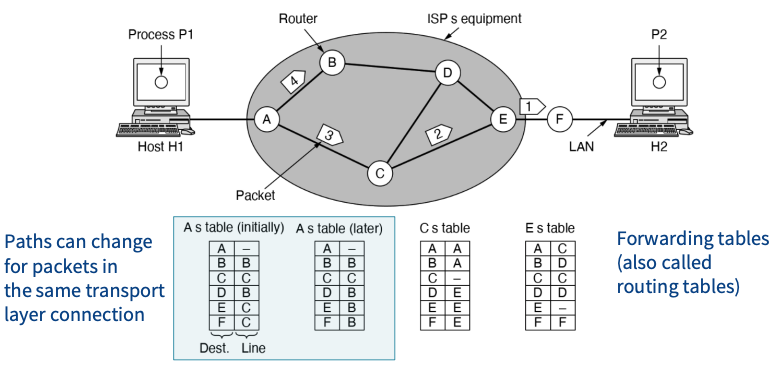
\includegraphics[width=\linewidth]{figs/packet-forwarding-connectionless.png}\\
\textbf{Packet forwarding (connection-oriented):} uses circuit switching and called virtual circuit network.\\
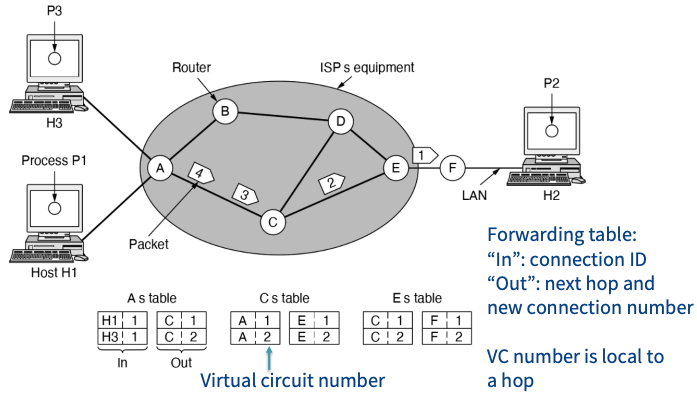
\includegraphics[width=\linewidth]{figs/packet-forwarding-connection-oriented.png}\\

\section{W11-12: Network Layer}


% % You can even have references
% \rule{0.3\linewidth}{0.25pt}
% \scriptsize
% \bibliographystyle{abstract}
% \bibliography{refFile}
\end{multicols}
\end{document}